\documentclass[1p]{elsarticle_modified}
%\bibliographystyle{elsarticle-num}

%\usepackage[colorlinks]{hyperref}
%\usepackage{abbrmath_seonhwa} %\Abb, \Ascr, \Acal ,\Abf, \Afrak
\usepackage{amsfonts}
\usepackage{amssymb}
\usepackage{amsmath}
\usepackage{amsthm}
\usepackage{scalefnt}
\usepackage{amsbsy}
\usepackage{kotex}
\usepackage{caption}
\usepackage{subfig}
\usepackage{color}
\usepackage{graphicx}
\usepackage{xcolor} %% white, black, red, green, blue, cyan, magenta, yellow
\usepackage{float}
\usepackage{setspace}
\usepackage{hyperref}

\usepackage{tikz}
\usetikzlibrary{arrows}

\usepackage{multirow}
\usepackage{array} % fixed length table
\usepackage{hhline}

%%%%%%%%%%%%%%%%%%%%%
\makeatletter
\renewcommand*\env@matrix[1][\arraystretch]{%
	\edef\arraystretch{#1}%
	\hskip -\arraycolsep
	\let\@ifnextchar\new@ifnextchar
	\array{*\c@MaxMatrixCols c}}
\makeatother %https://tex.stackexchange.com/questions/14071/how-can-i-increase-the-line-spacing-in-a-matrix
%%%%%%%%%%%%%%%

\usepackage[normalem]{ulem}

\newcommand{\msout}[1]{\ifmmode\text{\sout{\ensuremath{#1}}}\else\sout{#1}\fi}
%SOURCE: \msout is \stkout macro in https://tex.stackexchange.com/questions/20609/strikeout-in-math-mode

\newcommand{\cancel}[1]{
	\ifmmode
	{\color{red}\msout{#1}}
	\else
	{\color{red}\sout{#1}}
	\fi
}

\newcommand{\add}[1]{
	{\color{blue}\uwave{#1}}
}

\newcommand{\replace}[2]{
	\ifmmode
	{\color{red}\msout{#1}}{\color{blue}\uwave{#2}}
	\else
	{\color{red}\sout{#1}}{\color{blue}\uwave{#2}}
	\fi
}

\newcommand{\Sol}{\mathcal{S}} %segment
\newcommand{\D}{D} %diagram
\newcommand{\A}{\mathcal{A}} %arc


%%%%%%%%%%%%%%%%%%%%%%%%%%%%%5 test

\def\sl{\operatorname{\textup{SL}}(2,\Cbb)}
\def\psl{\operatorname{\textup{PSL}}(2,\Cbb)}
\def\quan{\mkern 1mu \triangleright \mkern 1mu}

\theoremstyle{definition}
\newtheorem{thm}{Theorem}[section]
\newtheorem{prop}[thm]{Proposition}
\newtheorem{lem}[thm]{Lemma}
\newtheorem{ques}[thm]{Question}
\newtheorem{cor}[thm]{Corollary}
\newtheorem{defn}[thm]{Definition}
\newtheorem{exam}[thm]{Example}
\newtheorem{rmk}[thm]{Remark}
\newtheorem{alg}[thm]{Algorithm}

\newcommand{\I}{\sqrt{-1}}
\begin{document}

%\begin{frontmatter}
%
%\title{Boundary parabolic representations of knots up to 8 crossings}
%
%%% Group authors per affiliation:
%\author{Yunhi Cho} 
%\address{Department of Mathematics, University of Seoul, Seoul, Korea}
%\ead{yhcho@uos.ac.kr}
%
%
%\author{Seonhwa Kim} %\fnref{s_kim}}
%\address{Center for Geometry and Physics, Institute for Basic Science, Pohang, 37673, Korea}
%\ead{ryeona17@ibs.re.kr}
%
%\author{Hyuk Kim}
%\address{Department of Mathematical Sciences, Seoul National University, Seoul 08826, Korea}
%\ead{hyukkim@snu.ac.kr}
%
%\author{Seokbeom Yoon}
%\address{Department of Mathematical Sciences, Seoul National University, Seoul, 08826,  Korea}
%\ead{sbyoon15@snu.ac.kr}
%
%\begin{abstract}
%We find all boundary parabolic representation of knots up to 8 crossings.
%
%\end{abstract}
%\begin{keyword}
%    \MSC[2010] 57M25 
%\end{keyword}
%
%\end{frontmatter}

%\linenumbers
%\tableofcontents
%
\newcommand\colored[1]{\textcolor{white}{\rule[-0.35ex]{0.8em}{1.4ex}}\kern-0.8em\color{red} #1}%
%\newcommand\colored[1]{\textcolor{white}{ #1}\kern-2.17ex	\textcolor{white}{ #1}\kern-1.81ex	\textcolor{white}{ #1}\kern-2.15ex\color{red}#1	}

{\Large $\underline{12a_{0001}~(K12a_{0001})}$}

\setlength{\tabcolsep}{10pt}
\renewcommand{\arraystretch}{1.6}
\vspace{1cm}\begin{tabular}{m{100pt}>{\centering\arraybackslash}m{274pt}}
\multirow{5}{120pt}{
	\centering
	\includegraphics[width=112pt]{../../../GIT/diagram.site/Diagrams/png/802_12a_0001.png}\\
\ \ \ A knot diagram\footnotemark}&
\allowdisplaybreaks
\textbf{Linearized knot diagam} \\
\cline{2-2}
 &
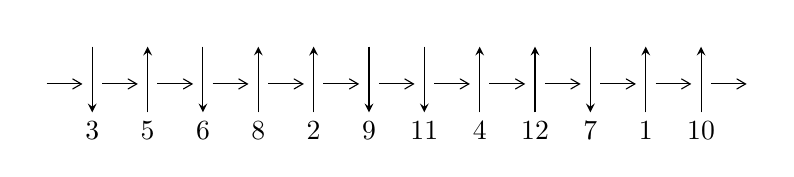
\begin{tikzpicture}[x=20pt, y=17pt]
	% nodes
	\node (C0) at (0, 0) {};
	\node (C1) at (1, 0) {};
	\node (C1U) at (1, +1) {};
	\node (C1D) at (1, -1) {3};

	\node (C2) at (2, 0) {};
	\node (C2U) at (2, +1) {};
	\node (C2D) at (2, -1) {5};

	\node (C3) at (3, 0) {};
	\node (C3U) at (3, +1) {};
	\node (C3D) at (3, -1) {6};

	\node (C4) at (4, 0) {};
	\node (C4U) at (4, +1) {};
	\node (C4D) at (4, -1) {8};

	\node (C5) at (5, 0) {};
	\node (C5U) at (5, +1) {};
	\node (C5D) at (5, -1) {2};

	\node (C6) at (6, 0) {};
	\node (C6U) at (6, +1) {};
	\node (C6D) at (6, -1) {9};

	\node (C7) at (7, 0) {};
	\node (C7U) at (7, +1) {};
	\node (C7D) at (7, -1) {11};

	\node (C8) at (8, 0) {};
	\node (C8U) at (8, +1) {};
	\node (C8D) at (8, -1) {4};

	\node (C9) at (9, 0) {};
	\node (C9U) at (9, +1) {};
	\node (C9D) at (9, -1) {12};

	\node (C10) at (10, 0) {};
	\node (C10U) at (10, +1) {};
	\node (C10D) at (10, -1) {7};

	\node (C11) at (11, 0) {};
	\node (C11U) at (11, +1) {};
	\node (C11D) at (11, -1) {1};

	\node (C12) at (12, 0) {};
	\node (C12U) at (12, +1) {};
	\node (C12D) at (12, -1) {10};
	\node (C13) at (13, 0) {};

	% arrows
	\draw[->,>={angle 60}]
	(C0) edge (C1) (C1) edge (C2) (C2) edge (C3) (C3) edge (C4) (C4) edge (C5) (C5) edge (C6) (C6) edge (C7) (C7) edge (C8) (C8) edge (C9) (C9) edge (C10) (C10) edge (C11) (C11) edge (C12) (C12) edge (C13) ;	\draw[->,>=stealth]
	(C1U) edge (C1D) (C2D) edge (C2U) (C3U) edge (C3D) (C4D) edge (C4U) (C5D) edge (C5U) (C6U) edge (C6D) (C7U) edge (C7D) (C8D) edge (C8U) (C9D) edge (C9U) (C10U) edge (C10D) (C11D) edge (C11U) (C12D) edge (C12U) ;
	\end{tikzpicture} \\
\hhline{~~} \\& 
\textbf{Solving Sequence} \\ \cline{2-2} 
 &
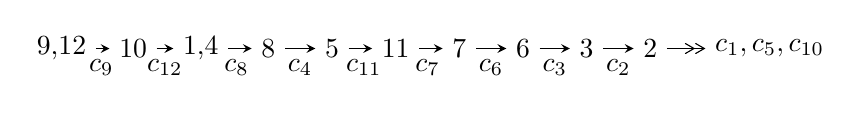
\begin{tikzpicture}[x=23pt, y=7pt]
	% node
	\node (A0) at (-1/8, 0) {9,12};
	\node (A1) at (1, 0) {10};
	\node (A2) at (33/16, 0) {1,4};
	\node (A3) at (25/8, 0) {8};
	\node (A4) at (33/8, 0) {5};
	\node (A5) at (41/8, 0) {11};
	\node (A6) at (49/8, 0) {7};
	\node (A7) at (57/8, 0) {6};
	\node (A8) at (65/8, 0) {3};
	\node (A9) at (73/8, 0) {2};
	\node (C1) at (1/2, -1) {$c_{9}$};
	\node (C2) at (3/2, -1) {$c_{12}$};
	\node (C3) at (21/8, -1) {$c_{8}$};
	\node (C4) at (29/8, -1) {$c_{4}$};
	\node (C5) at (37/8, -1) {$c_{11}$};
	\node (C6) at (45/8, -1) {$c_{7}$};
	\node (C7) at (53/8, -1) {$c_{6}$};
	\node (C8) at (61/8, -1) {$c_{3}$};
	\node (C9) at (69/8, -1) {$c_{2}$};
	\node (A10) at (11, 0) {$c_{1},c_{5},c_{10}$};

	% edge
	\draw[->,>=stealth]	
	(A0) edge (A1) (A1) edge (A2) (A2) edge (A3) (A3) edge (A4) (A4) edge (A5) (A5) edge (A6) (A6) edge (A7) (A7) edge (A8) (A8) edge (A9) ;
	\draw[->>,>={angle 60}]	
	(A9) edge (A10);
\end{tikzpicture} \\ 

\end{tabular} \\

\footnotetext{
The image of knot diagram is generated by the software ``\textbf{Draw programme}" developed by Andrew Bartholomew(\url{http://www.layer8.co.uk/maths/draw/index.htm\#Running-draw}), where we modified some parts for our purpose(\url{https://github.com/CATsTAILs/LinksPainter}).
}\phantom \\ \newline 
\centering \textbf{Ideals for irreducible components\footnotemark of $X_{\text{par}}$} 
 
\begin{align*}
I^u_{1}&=\langle 
3.90724\times10^{78} u^{127}-4.51726\times10^{79} u^{126}+\cdots+5.58481\times10^{75} b-1.43118\times10^{78},\\
\phantom{I^u_{1}}&\phantom{= \langle  }4.97117\times10^{78} u^{127}-5.50418\times10^{79} u^{126}+\cdots+5.58481\times10^{75} a+9.59232\times10^{77},\;u^{128}-13 u^{127}+\cdots-3 u+1\rangle \\
I^u_{2}&=\langle 
b,\;- u^5+u^3 a+2 u^4- u^2 a+a^2-2 u^2+a+u,\;u^6- u^5- u^4+2 u^3- u+1\rangle \\
I^u_{3}&=\langle 
a^2+b+a-1,\;a^4+a^3-2 a^2- a+2,\;u+1\rangle \\
I^u_{4}&=\langle 
a^5-3 a^4+4 a^2+b+a-1,\;a^6-3 a^5+5 a^3- a^2-2 a+1,\;u+1\rangle \\
\\
\end{align*}
\raggedright * 4 irreducible components of $\dim_{\mathbb{C}}=0$, with total 150 representations.\\
\footnotetext{All coefficients of polynomials are rational numbers. But the coefficients are sometimes approximated in decimal forms when there is not enough margin.}
\newpage
\renewcommand{\arraystretch}{1}
\centering \section*{I. $I^u_{1}= \langle 3.91\times10^{78} u^{127}-4.52\times10^{79} u^{126}+\cdots+5.58\times10^{75} b-1.43\times10^{78},\;4.97\times10^{78} u^{127}-5.50\times10^{79} u^{126}+\cdots+5.58\times10^{75} a+9.59\times10^{77},\;u^{128}-13 u^{127}+\cdots-3 u+1 \rangle$}
\flushleft \textbf{(i) Arc colorings}\\
\begin{tabular}{m{7pt} m{180pt} m{7pt} m{180pt} }
\flushright $a_{9}=$&$\begin{pmatrix}1\\0\end{pmatrix}$ \\
\flushright $a_{12}=$&$\begin{pmatrix}0\\u\end{pmatrix}$ \\
\flushright $a_{10}=$&$\begin{pmatrix}1\\- u^2\end{pmatrix}$ \\
\flushright $a_{1}=$&$\begin{pmatrix}u\\- u^3+u\end{pmatrix}$ \\
\flushright $a_{4}=$&$\begin{pmatrix}-890.124 u^{127}+9855.63 u^{126}+\cdots-533.258 u-171.757\\-699.620 u^{127}+8088.48 u^{126}+\cdots-995.384 u+256.262\end{pmatrix}$ \\
\flushright $a_{8}=$&$\begin{pmatrix}726.036 u^{127}-9831.86 u^{126}+\cdots+2699.13 u-1698.98\\534.963 u^{127}-4792.44 u^{126}+\cdots-933.777 u+1212.53\end{pmatrix}$ \\
\flushright $a_{5}=$&$\begin{pmatrix}-1886.04 u^{127}+22618.7 u^{126}+\cdots-3435.20 u+1391.46\\-473.156 u^{127}+3944.04 u^{126}+\cdots+1228.16 u-1364.18\end{pmatrix}$ \\
\flushright $a_{11}=$&$\begin{pmatrix}- u^3\\u^5- u^3+u\end{pmatrix}$ \\
\flushright $a_{7}=$&$\begin{pmatrix}1184.26 u^{127}-16846.3 u^{126}+\cdots+5432.79 u-3580.45\\421.670 u^{127}-3154.11 u^{126}+\cdots-1503.13 u+1602.68\end{pmatrix}$ \\
\flushright $a_{6}=$&$\begin{pmatrix}1605.93 u^{127}-20000.5 u^{126}+\cdots+3929.65 u-1977.77\\421.670 u^{127}-3154.11 u^{126}+\cdots-1503.13 u+1602.68\end{pmatrix}$ \\
\flushright $a_{3}=$&$\begin{pmatrix}-1994.18 u^{127}+23589.1 u^{126}+\cdots-3282.53 u+1117.67\\-165.031 u^{127}+388.300 u^{126}+\cdots+1669.75 u-1431.77\end{pmatrix}$ \\
\flushright $a_{2}=$&$\begin{pmatrix}-1938.13 u^{127}+22466.1 u^{126}+\cdots-2775.51 u+659.657\\490.496 u^{127}-6640.18 u^{126}+\cdots+1926.70 u-1129.42\end{pmatrix}$\\&\end{tabular}
\flushleft \textbf{(ii) Obstruction class $= -1$}\\~\\
\flushleft \textbf{(iii) Cusp Shapes $= -4093.96 u^{127}+45529.3 u^{126}+\cdots-3370.47 u-481.481$}\\~\\
\newpage\renewcommand{\arraystretch}{1}
\flushleft \textbf{(iv) u-Polynomials at the component}\newline \\
\begin{tabular}{m{50pt}|m{274pt}}
Crossings & \hspace{64pt}u-Polynomials at each crossing \\
\hline $$\begin{aligned}c_{1}\end{aligned}$$&$\begin{aligned}
&u^{128}+64 u^{127}+\cdots+8 u+1
\end{aligned}$\\
\hline $$\begin{aligned}c_{2},c_{5}\end{aligned}$$&$\begin{aligned}
&u^{128}+8 u^{127}+\cdots+8 u+1
\end{aligned}$\\
\hline $$\begin{aligned}c_{3}\end{aligned}$$&$\begin{aligned}
&u^{128}-8 u^{127}+\cdots-97068 u+41508
\end{aligned}$\\
\hline $$\begin{aligned}c_{4},c_{8}\end{aligned}$$&$\begin{aligned}
&u^{128}-2 u^{127}+\cdots+8192 u+4096
\end{aligned}$\\
\hline $$\begin{aligned}c_{6}\end{aligned}$$&$\begin{aligned}
&u^{128}-4 u^{127}+\cdots-59111052 u+3579401
\end{aligned}$\\
\hline $$\begin{aligned}c_{7},c_{10}\end{aligned}$$&$\begin{aligned}
&u^{128}+3 u^{127}+\cdots+6144 u+1024
\end{aligned}$\\
\hline $$\begin{aligned}c_{9},c_{12}\end{aligned}$$&$\begin{aligned}
&u^{128}+13 u^{127}+\cdots+3 u+1
\end{aligned}$\\
\hline $$\begin{aligned}c_{11}\end{aligned}$$&$\begin{aligned}
&u^{128}-59 u^{127}+\cdots+37 u+1
\end{aligned}$\\
\hline
\end{tabular}\\~\\
\newpage\renewcommand{\arraystretch}{1}
\flushleft \textbf{(v) Riley Polynomials at the component}\newline \\
\begin{tabular}{m{50pt}|m{274pt}}
Crossings & \hspace{64pt}Riley Polynomials at each crossing \\
\hline $$\begin{aligned}c_{1}\end{aligned}$$&$\begin{aligned}
&y^{128}+8 y^{127}+\cdots+64 y+1
\end{aligned}$\\
\hline $$\begin{aligned}c_{2},c_{5}\end{aligned}$$&$\begin{aligned}
&y^{128}+64 y^{127}+\cdots+8 y+1
\end{aligned}$\\
\hline $$\begin{aligned}c_{3}\end{aligned}$$&$\begin{aligned}
&y^{128}-48 y^{127}+\cdots+110992594392 y+1722914064
\end{aligned}$\\
\hline $$\begin{aligned}c_{4},c_{8}\end{aligned}$$&$\begin{aligned}
&y^{128}+70 y^{127}+\cdots+520093696 y+16777216
\end{aligned}$\\
\hline $$\begin{aligned}c_{6}\end{aligned}$$&$\begin{aligned}
&y^{128}-56 y^{127}+\cdots-158438371667520 y+12812111518801
\end{aligned}$\\
\hline $$\begin{aligned}c_{7},c_{10}\end{aligned}$$&$\begin{aligned}
&y^{128}-69 y^{127}+\cdots-27787264 y+1048576
\end{aligned}$\\
\hline $$\begin{aligned}c_{9},c_{12}\end{aligned}$$&$\begin{aligned}
&y^{128}-59 y^{127}+\cdots+37 y+1
\end{aligned}$\\
\hline $$\begin{aligned}c_{11}\end{aligned}$$&$\begin{aligned}
&y^{128}+33 y^{127}+\cdots-4663 y+1
\end{aligned}$\\
\hline
\end{tabular}\\~\\
\newpage\flushleft \textbf{(vi) Complex Volumes and Cusp Shapes}
$$\begin{array}{c|c|c}  
\text{Solutions to }I^u_{1}& \I (\text{vol} + \sqrt{-1}CS) & \text{Cusp shape}\\
 \hline 
\begin{aligned}
u &= \phantom{-}0.467216 + 0.888765 I \\
a &= -0.262139 - 0.326352 I \\
b &= -1.174290 - 0.314881 I\end{aligned}
 & -5.57599 - 5.97894 I & \phantom{-0.000000 } 0 \\ \hline\begin{aligned}
u &= \phantom{-}0.467216 - 0.888765 I \\
a &= -0.262139 + 0.326352 I \\
b &= -1.174290 + 0.314881 I\end{aligned}
 & -5.57599 + 5.97894 I & \phantom{-0.000000 } 0 \\ \hline\begin{aligned}
u &= \phantom{-}0.884815 + 0.447263 I \\
a &= \phantom{-}0.736525 + 0.098393 I \\
b &= -0.646072 + 0.807347 I\end{aligned}
 & \phantom{-}1.78444 + 0.33658 I & \phantom{-0.000000 } 0 \\ \hline\begin{aligned}
u &= \phantom{-}0.884815 - 0.447263 I \\
a &= \phantom{-}0.736525 - 0.098393 I \\
b &= -0.646072 - 0.807347 I\end{aligned}
 & \phantom{-}1.78444 - 0.33658 I & \phantom{-0.000000 } 0 \\ \hline\begin{aligned}
u &= \phantom{-}0.903432 + 0.456730 I \\
a &= \phantom{-}1.332140 - 0.440260 I \\
b &= -0.785831 - 0.652425 I\end{aligned}
 & \phantom{-}1.86792 + 3.29651 I & \phantom{-0.000000 } 0 \\ \hline\begin{aligned}
u &= \phantom{-}0.903432 - 0.456730 I \\
a &= \phantom{-}1.332140 + 0.440260 I \\
b &= -0.785831 + 0.652425 I\end{aligned}
 & \phantom{-}1.86792 - 3.29651 I & \phantom{-0.000000 } 0 \\ \hline\begin{aligned}
u &= \phantom{-}0.549415 + 0.856556 I \\
a &= -0.314902 - 0.196049 I \\
b &= -1.170170 + 0.054456 I\end{aligned}
 & -6.12700 + 1.81309 I & \phantom{-0.000000 } 0 \\ \hline\begin{aligned}
u &= \phantom{-}0.549415 - 0.856556 I \\
a &= -0.314902 + 0.196049 I \\
b &= -1.170170 - 0.054456 I\end{aligned}
 & -6.12700 - 1.81309 I & \phantom{-0.000000 } 0 \\ \hline\begin{aligned}
u &= \phantom{-}0.421809 + 0.932088 I \\
a &= -0.16666 - 1.56984 I \\
b &= \phantom{-}0.574257 - 1.264840 I\end{aligned}
 & -6.12043 - 7.30221 I & \phantom{-0.000000 } 0 \\ \hline\begin{aligned}
u &= \phantom{-}0.421809 - 0.932088 I \\
a &= -0.16666 + 1.56984 I \\
b &= \phantom{-}0.574257 + 1.264840 I\end{aligned}
 & -6.12043 + 7.30221 I & \phantom{-0.000000 } 0\\
 \hline 
 \end{array}$$\newpage$$\begin{array}{c|c|c}  
\text{Solutions to }I^u_{1}& \I (\text{vol} + \sqrt{-1}CS) & \text{Cusp shape}\\
 \hline 
\begin{aligned}
u &= \phantom{-}0.465799 + 0.851706 I \\
a &= -0.17541 - 2.04875 I \\
b &= \phantom{-}0.259022 - 1.027760 I\end{aligned}
 & -3.31867 - 4.55381 I & \phantom{-0.000000 } 0 \\ \hline\begin{aligned}
u &= \phantom{-}0.465799 - 0.851706 I \\
a &= -0.17541 + 2.04875 I \\
b &= \phantom{-}0.259022 + 1.027760 I\end{aligned}
 & -3.31867 + 4.55381 I & \phantom{-0.000000 } 0 \\ \hline\begin{aligned}
u &= -0.926528 + 0.448937 I \\
a &= -0.503695 + 0.895385 I \\
b &= -0.775401 - 0.266682 I\end{aligned}
 & \phantom{-}1.78403 - 1.66122 I & \phantom{-0.000000 } 0 \\ \hline\begin{aligned}
u &= -0.926528 - 0.448937 I \\
a &= -0.503695 - 0.895385 I \\
b &= -0.775401 + 0.266682 I\end{aligned}
 & \phantom{-}1.78403 + 1.66122 I & \phantom{-0.000000 } 0 \\ \hline\begin{aligned}
u &= \phantom{-}0.506875 + 0.826946 I \\
a &= -0.08559 + 2.23069 I \\
b &= -0.064227 + 0.999070 I\end{aligned}
 & -3.61244 + 0.86916 I & \phantom{-0.000000 } 0 \\ \hline\begin{aligned}
u &= \phantom{-}0.506875 - 0.826946 I \\
a &= -0.08559 - 2.23069 I \\
b &= -0.064227 - 0.999070 I\end{aligned}
 & -3.61244 - 0.86916 I & \phantom{-0.000000 } 0 \\ \hline\begin{aligned}
u &= -0.737819 + 0.621082 I \\
a &= \phantom{-}0.93612 + 2.04262 I \\
b &= \phantom{-}0.268137 + 1.346520 I\end{aligned}
 & -6.39276 - 1.42340 I & \phantom{-0.000000 } 0 \\ \hline\begin{aligned}
u &= -0.737819 - 0.621082 I \\
a &= \phantom{-}0.93612 - 2.04262 I \\
b &= \phantom{-}0.268137 - 1.346520 I\end{aligned}
 & -6.39276 + 1.42340 I & \phantom{-0.000000 } 0 \\ \hline\begin{aligned}
u &= \phantom{-}0.408451 + 0.952232 I \\
a &= \phantom{-}0.14412 + 1.47260 I \\
b &= -0.66863 + 1.31884 I\end{aligned}
 & -8.8015 - 12.5693 I & \phantom{-0.000000 } 0 \\ \hline\begin{aligned}
u &= \phantom{-}0.408451 - 0.952232 I \\
a &= \phantom{-}0.14412 - 1.47260 I \\
b &= -0.66863 - 1.31884 I\end{aligned}
 & -8.8015 + 12.5693 I & \phantom{-0.000000 } 0\\
 \hline 
 \end{array}$$\newpage$$\begin{array}{c|c|c}  
\text{Solutions to }I^u_{1}& \I (\text{vol} + \sqrt{-1}CS) & \text{Cusp shape}\\
 \hline 
\begin{aligned}
u &= -0.862643 + 0.428421 I \\
a &= -1.21199 - 2.91585 I \\
b &= \phantom{-}0.062599 - 0.793471 I\end{aligned}
 & \phantom{-}1.108160 + 0.710643 I & \phantom{-0.000000 } 0 \\ \hline\begin{aligned}
u &= -0.862643 - 0.428421 I \\
a &= -1.21199 + 2.91585 I \\
b &= \phantom{-}0.062599 + 0.793471 I\end{aligned}
 & \phantom{-}1.108160 - 0.710643 I & \phantom{-0.000000 } 0 \\ \hline\begin{aligned}
u &= -0.919358 + 0.483575 I \\
a &= \phantom{-}1.59445 + 2.58825 I \\
b &= -0.285476 + 0.894692 I\end{aligned}
 & \phantom{-}1.44266 - 4.40723 I & \phantom{-0.000000 } 0 \\ \hline\begin{aligned}
u &= -0.919358 - 0.483575 I \\
a &= \phantom{-}1.59445 - 2.58825 I \\
b &= -0.285476 - 0.894692 I\end{aligned}
 & \phantom{-}1.44266 + 4.40723 I & \phantom{-0.000000 } 0 \\ \hline\begin{aligned}
u &= \phantom{-}0.918229 + 0.497793 I \\
a &= -0.788010 - 0.432152 I \\
b &= \phantom{-}0.615333 - 0.754332 I\end{aligned}
 & \phantom{-}0.54839 + 5.39329 I & \phantom{-0.000000 } 0 \\ \hline\begin{aligned}
u &= \phantom{-}0.918229 - 0.497793 I \\
a &= -0.788010 + 0.432152 I \\
b &= \phantom{-}0.615333 + 0.754332 I\end{aligned}
 & \phantom{-}0.54839 - 5.39329 I & \phantom{-0.000000 } 0 \\ \hline\begin{aligned}
u &= \phantom{-}0.472353 + 0.826605 I \\
a &= \phantom{-}0.199203 + 0.250333 I \\
b &= \phantom{-}0.943077 + 0.193062 I\end{aligned}
 & -2.84693 - 1.72799 I & \phantom{-0.000000 } 0 \\ \hline\begin{aligned}
u &= \phantom{-}0.472353 - 0.826605 I \\
a &= \phantom{-}0.199203 - 0.250333 I \\
b &= \phantom{-}0.943077 - 0.193062 I\end{aligned}
 & -2.84693 + 1.72799 I & \phantom{-0.000000 } 0 \\ \hline\begin{aligned}
u &= \phantom{-}0.460270 + 0.946554 I \\
a &= \phantom{-}0.01204 + 1.62062 I \\
b &= -0.44420 + 1.39719 I\end{aligned}
 & -11.01500 - 3.84928 I & \phantom{-0.000000 } 0 \\ \hline\begin{aligned}
u &= \phantom{-}0.460270 - 0.946554 I \\
a &= \phantom{-}0.01204 - 1.62062 I \\
b &= -0.44420 - 1.39719 I\end{aligned}
 & -11.01500 + 3.84928 I & \phantom{-0.000000 } 0\\
 \hline 
 \end{array}$$\newpage$$\begin{array}{c|c|c}  
\text{Solutions to }I^u_{1}& \I (\text{vol} + \sqrt{-1}CS) & \text{Cusp shape}\\
 \hline 
\begin{aligned}
u &= \phantom{-}0.831926 + 0.448912 I \\
a &= -1.55091 + 0.63092 I \\
b &= \phantom{-}0.825714 + 0.605979 I\end{aligned}
 & \phantom{-}0.17233 - 1.51959 I & \phantom{-0.000000 } 0 \\ \hline\begin{aligned}
u &= \phantom{-}0.831926 - 0.448912 I \\
a &= -1.55091 - 0.63092 I \\
b &= \phantom{-}0.825714 - 0.605979 I\end{aligned}
 & \phantom{-}0.17233 + 1.51959 I & \phantom{-0.000000 } 0 \\ \hline\begin{aligned}
u &= -0.910580 + 0.533390 I \\
a &= \phantom{-}0.623441 - 1.010220 I \\
b &= \phantom{-}1.072100 + 0.299027 I\end{aligned}
 & -0.61836 - 5.74521 I & \phantom{-0.000000 } 0 \\ \hline\begin{aligned}
u &= -0.910580 - 0.533390 I \\
a &= \phantom{-}0.623441 + 1.010220 I \\
b &= \phantom{-}1.072100 - 0.299027 I\end{aligned}
 & -0.61836 + 5.74521 I & \phantom{-0.000000 } 0 \\ \hline\begin{aligned}
u &= -1.056700 + 0.121003 I \\
a &= \phantom{-}1.40180 - 2.12162 I \\
b &= -0.246674 - 0.447064 I\end{aligned}
 & \phantom{-}1.97936 - 2.35936 I & \phantom{-0.000000 } 0 \\ \hline\begin{aligned}
u &= -1.056700 - 0.121003 I \\
a &= \phantom{-}1.40180 + 2.12162 I \\
b &= -0.246674 + 0.447064 I\end{aligned}
 & \phantom{-}1.97936 + 2.35936 I & \phantom{-0.000000 } 0 \\ \hline\begin{aligned}
u &= -0.782301 + 0.501067 I \\
a &= \phantom{-}0.514821 - 1.161720 I \\
b &= \phantom{-}1.024760 - 0.105409 I\end{aligned}
 & -1.05662 + 1.51276 I & \phantom{-0.000000 } 0 \\ \hline\begin{aligned}
u &= -0.782301 - 0.501067 I \\
a &= \phantom{-}0.514821 + 1.161720 I \\
b &= \phantom{-}1.024760 + 0.105409 I\end{aligned}
 & -1.05662 - 1.51276 I & \phantom{-0.000000 } 0 \\ \hline\begin{aligned}
u &= \phantom{-}0.637614 + 0.871450 I \\
a &= -0.50478 + 1.83058 I \\
b &= \phantom{-}0.380560 + 1.312160 I\end{aligned}
 & -7.55837 + 2.76750 I & \phantom{-0.000000 } 0 \\ \hline\begin{aligned}
u &= \phantom{-}0.637614 - 0.871450 I \\
a &= -0.50478 - 1.83058 I \\
b &= \phantom{-}0.380560 - 1.312160 I\end{aligned}
 & -7.55837 - 2.76750 I & \phantom{-0.000000 } 0\\
 \hline 
 \end{array}$$\newpage$$\begin{array}{c|c|c}  
\text{Solutions to }I^u_{1}& \I (\text{vol} + \sqrt{-1}CS) & \text{Cusp shape}\\
 \hline 
\begin{aligned}
u &= \phantom{-}0.664691 + 0.620912 I \\
a &= \phantom{-}0.0740313 - 0.0478021 I \\
b &= \phantom{-}0.641222 - 0.618829 I\end{aligned}
 & -3.24131 + 0.01631 I & \phantom{-0.000000 } 0 \\ \hline\begin{aligned}
u &= \phantom{-}0.664691 - 0.620912 I \\
a &= \phantom{-}0.0740313 + 0.0478021 I \\
b &= \phantom{-}0.641222 + 0.618829 I\end{aligned}
 & -3.24131 - 0.01631 I & \phantom{-0.000000 } 0 \\ \hline\begin{aligned}
u &= -0.642929 + 0.634338 I \\
a &= \phantom{-}0.70955 + 1.92950 I \\
b &= \phantom{-}0.539215 + 1.287990 I\end{aligned}
 & -4.76631 + 7.04658 I & \phantom{-0.000000 } 0 \\ \hline\begin{aligned}
u &= -0.642929 - 0.634338 I \\
a &= \phantom{-}0.70955 - 1.92950 I \\
b &= \phantom{-}0.539215 - 1.287990 I\end{aligned}
 & -4.76631 - 7.04658 I & \phantom{-0.000000 } 0 \\ \hline\begin{aligned}
u &= \phantom{-}0.608648 + 0.912650 I \\
a &= \phantom{-}0.39418 - 1.78668 I \\
b &= -0.23220 - 1.45855 I\end{aligned}
 & -12.00690 - 1.08932 I & \phantom{-0.000000 } 0 \\ \hline\begin{aligned}
u &= \phantom{-}0.608648 - 0.912650 I \\
a &= \phantom{-}0.39418 + 1.78668 I \\
b &= -0.23220 + 1.45855 I\end{aligned}
 & -12.00690 + 1.08932 I & \phantom{-0.000000 } 0 \\ \hline\begin{aligned}
u &= -0.926319 + 0.604861 I \\
a &= -1.47167 - 2.09294 I \\
b &= \phantom{-}0.394748 - 1.334950 I\end{aligned}
 & -5.81461 - 3.40517 I & \phantom{-0.000000 } 0 \\ \hline\begin{aligned}
u &= -0.926319 - 0.604861 I \\
a &= -1.47167 + 2.09294 I \\
b &= \phantom{-}0.394748 + 1.334950 I\end{aligned}
 & -5.81461 + 3.40517 I & \phantom{-0.000000 } 0 \\ \hline\begin{aligned}
u &= \phantom{-}0.929829 + 0.599892 I \\
a &= -0.826514 + 0.810044 I \\
b &= \phantom{-}0.838781 + 0.511078 I\end{aligned}
 & -2.49531 + 4.79440 I & \phantom{-0.000000 } 0 \\ \hline\begin{aligned}
u &= \phantom{-}0.929829 - 0.599892 I \\
a &= -0.826514 - 0.810044 I \\
b &= \phantom{-}0.838781 - 0.511078 I\end{aligned}
 & -2.49531 - 4.79440 I & \phantom{-0.000000 } 0\\
 \hline 
 \end{array}$$\newpage$$\begin{array}{c|c|c}  
\text{Solutions to }I^u_{1}& \I (\text{vol} + \sqrt{-1}CS) & \text{Cusp shape}\\
 \hline 
\begin{aligned}
u &= \phantom{-}0.834599 + 0.317293 I \\
a &= \phantom{-}0.607611 - 0.429842 I \\
b &= -0.607666 + 0.987525 I\end{aligned}
 & \phantom{-}0.79205 - 1.96703 I & \phantom{-0.000000 } 0 \\ \hline\begin{aligned}
u &= \phantom{-}0.834599 - 0.317293 I \\
a &= \phantom{-}0.607611 + 0.429842 I \\
b &= -0.607666 - 0.987525 I\end{aligned}
 & \phantom{-}0.79205 + 1.96703 I & \phantom{-0.000000 } 0 \\ \hline\begin{aligned}
u &= \phantom{-}0.848804 + 0.266513 I \\
a &= -0.632048 + 0.603499 I \\
b &= \phantom{-}0.613884 - 1.086290 I\end{aligned}
 & -1.41894 - 6.93011 I & \phantom{-0.000000 } 0 \\ \hline\begin{aligned}
u &= \phantom{-}0.848804 - 0.266513 I \\
a &= -0.632048 - 0.603499 I \\
b &= \phantom{-}0.613884 + 1.086290 I\end{aligned}
 & -1.41894 + 6.93011 I & \phantom{-0.000000 } 0 \\ \hline\begin{aligned}
u &= -0.667096 + 0.585551 I \\
a &= -0.72206 - 2.07304 I \\
b &= -0.429340 - 1.193630 I\end{aligned}
 & -2.01099 + 2.08594 I & \phantom{-0.000000 } 0 \\ \hline\begin{aligned}
u &= -0.667096 - 0.585551 I \\
a &= -0.72206 + 2.07304 I \\
b &= -0.429340 + 1.193630 I\end{aligned}
 & -2.01099 - 2.08594 I & \phantom{-0.000000 } 0 \\ \hline\begin{aligned}
u &= \phantom{-}0.671246 + 0.887919 I \\
a &= \phantom{-}0.52699 - 1.75239 I \\
b &= -0.50667 - 1.39349 I\end{aligned}
 & -10.56640 + 7.80081 I & \phantom{-0.000000 } 0 \\ \hline\begin{aligned}
u &= \phantom{-}0.671246 - 0.887919 I \\
a &= \phantom{-}0.52699 + 1.75239 I \\
b &= -0.50667 + 1.39349 I\end{aligned}
 & -10.56640 - 7.80081 I & \phantom{-0.000000 } 0 \\ \hline\begin{aligned}
u &= -1.040140 + 0.399543 I \\
a &= -0.640041 + 0.567994 I \\
b &= -0.394283 - 0.566210 I\end{aligned}
 & \phantom{-}2.19825 - 1.39363 I & \phantom{-0.000000 } 0 \\ \hline\begin{aligned}
u &= -1.040140 - 0.399543 I \\
a &= -0.640041 - 0.567994 I \\
b &= -0.394283 + 0.566210 I\end{aligned}
 & \phantom{-}2.19825 + 1.39363 I & \phantom{-0.000000 } 0\\
 \hline 
 \end{array}$$\newpage$$\begin{array}{c|c|c}  
\text{Solutions to }I^u_{1}& \I (\text{vol} + \sqrt{-1}CS) & \text{Cusp shape}\\
 \hline 
\begin{aligned}
u &= \phantom{-}1.016570 + 0.457027 I \\
a &= \phantom{-}1.032610 - 0.035620 I \\
b &= -0.575478 - 0.767072 I\end{aligned}
 & \phantom{-}1.86462 + 5.09781 I & \phantom{-0.000000 } 0 \\ \hline\begin{aligned}
u &= \phantom{-}1.016570 - 0.457027 I \\
a &= \phantom{-}1.032610 + 0.035620 I \\
b &= -0.575478 + 0.767072 I\end{aligned}
 & \phantom{-}1.86462 - 5.09781 I & \phantom{-0.000000 } 0 \\ \hline\begin{aligned}
u &= -0.965962 + 0.579568 I \\
a &= \phantom{-}1.61748 + 2.11047 I \\
b &= -0.544207 + 1.210720 I\end{aligned}
 & -1.10137 - 6.74666 I & \phantom{-0.000000 } 0 \\ \hline\begin{aligned}
u &= -0.965962 - 0.579568 I \\
a &= \phantom{-}1.61748 - 2.11047 I \\
b &= -0.544207 - 1.210720 I\end{aligned}
 & -1.10137 + 6.74666 I & \phantom{-0.000000 } 0 \\ \hline\begin{aligned}
u &= -0.983318 + 0.599046 I \\
a &= -1.62754 - 2.03045 I \\
b &= \phantom{-}0.63195 - 1.28165 I\end{aligned}
 & -3.74035 - 11.90180 I & \phantom{-0.000000 } 0 \\ \hline\begin{aligned}
u &= -0.983318 - 0.599046 I \\
a &= -1.62754 + 2.03045 I \\
b &= \phantom{-}0.63195 + 1.28165 I\end{aligned}
 & -3.74035 + 11.90180 I & \phantom{-0.000000 } 0 \\ \hline\begin{aligned}
u &= \phantom{-}1.065750 + 0.442801 I \\
a &= -0.997127 - 0.204455 I \\
b &= \phantom{-}0.456080 + 0.926673 I\end{aligned}
 & \phantom{-}0.00932 + 9.64129 I & \phantom{-0.000000 } 0 \\ \hline\begin{aligned}
u &= \phantom{-}1.065750 - 0.442801 I \\
a &= -0.997127 + 0.204455 I \\
b &= \phantom{-}0.456080 - 0.926673 I\end{aligned}
 & \phantom{-}0.00932 - 9.64129 I & \phantom{-0.000000 } 0 \\ \hline\begin{aligned}
u &= -1.162860 + 0.135909 I \\
a &= -1.323840 - 0.086207 I \\
b &= \phantom{-}0.645634 - 0.381020 I\end{aligned}
 & \phantom{-}2.61757 - 0.40705 I & \phantom{-0.000000 } 0 \\ \hline\begin{aligned}
u &= -1.162860 - 0.135909 I \\
a &= -1.323840 + 0.086207 I \\
b &= \phantom{-}0.645634 + 0.381020 I\end{aligned}
 & \phantom{-}2.61757 + 0.40705 I & \phantom{-0.000000 } 0\\
 \hline 
 \end{array}$$\newpage$$\begin{array}{c|c|c}  
\text{Solutions to }I^u_{1}& \I (\text{vol} + \sqrt{-1}CS) & \text{Cusp shape}\\
 \hline 
\begin{aligned}
u &= -1.150830 + 0.264016 I \\
a &= -1.040540 + 0.117585 I \\
b &= \phantom{-}0.346991 - 0.669629 I\end{aligned}
 & \phantom{-}2.55173 - 0.89115 I & \phantom{-0.000000 } 0 \\ \hline\begin{aligned}
u &= -1.150830 - 0.264016 I \\
a &= -1.040540 - 0.117585 I \\
b &= \phantom{-}0.346991 + 0.669629 I\end{aligned}
 & \phantom{-}2.55173 + 0.89115 I & \phantom{-0.000000 } 0 \\ \hline\begin{aligned}
u &= \phantom{-}0.347912 + 0.738078 I \\
a &= -0.054770 + 0.273114 I \\
b &= \phantom{-}0.424981 + 0.531973 I\end{aligned}
 & -1.87900 - 1.84140 I & \phantom{-0.000000 } 0 \\ \hline\begin{aligned}
u &= \phantom{-}0.347912 - 0.738078 I \\
a &= -0.054770 - 0.273114 I \\
b &= \phantom{-}0.424981 - 0.531973 I\end{aligned}
 & -1.87900 + 1.84140 I & \phantom{-0.000000 } 0 \\ \hline\begin{aligned}
u &= -1.181750 + 0.099439 I \\
a &= -0.883504 + 0.917778 I \\
b &= \phantom{-}0.300620 + 0.738938 I\end{aligned}
 & \phantom{-}2.43308 + 2.28422 I & \phantom{-0.000000 } 0 \\ \hline\begin{aligned}
u &= -1.181750 - 0.099439 I \\
a &= -0.883504 - 0.917778 I \\
b &= \phantom{-}0.300620 - 0.738938 I\end{aligned}
 & \phantom{-}2.43308 - 2.28422 I & \phantom{-0.000000 } 0 \\ \hline\begin{aligned}
u &= -1.142850 + 0.407232 I \\
a &= \phantom{-}0.938805 - 0.516089 I \\
b &= \phantom{-}0.189205 + 0.995087 I\end{aligned}
 & \phantom{-}0.18861 + 2.20753 I & \phantom{-0.000000 } 0 \\ \hline\begin{aligned}
u &= -1.142850 - 0.407232 I \\
a &= \phantom{-}0.938805 + 0.516089 I \\
b &= \phantom{-}0.189205 - 0.995087 I\end{aligned}
 & \phantom{-}0.18861 - 2.20753 I & \phantom{-0.000000 } 0 \\ \hline\begin{aligned}
u &= \phantom{-}1.118090 + 0.519341 I \\
a &= -0.561461 - 0.424753 I \\
b &= -0.082616 + 0.814985 I\end{aligned}
 & -0.91707 + 3.27060 I & \phantom{-0.000000 } 0 \\ \hline\begin{aligned}
u &= \phantom{-}1.118090 - 0.519341 I \\
a &= -0.561461 + 0.424753 I \\
b &= -0.082616 - 0.814985 I\end{aligned}
 & -0.91707 - 3.27060 I & \phantom{-0.000000 } 0\\
 \hline 
 \end{array}$$\newpage$$\begin{array}{c|c|c}  
\text{Solutions to }I^u_{1}& \I (\text{vol} + \sqrt{-1}CS) & \text{Cusp shape}\\
 \hline 
\begin{aligned}
u &= -1.202380 + 0.331291 I \\
a &= \phantom{-}1.105400 - 0.337621 I \\
b &= -0.266903 + 1.018850 I\end{aligned}
 & \phantom{-}0.37432 - 4.83030 I & \phantom{-0.000000 } 0 \\ \hline\begin{aligned}
u &= -1.202380 - 0.331291 I \\
a &= \phantom{-}1.105400 + 0.337621 I \\
b &= -0.266903 - 1.018850 I\end{aligned}
 & \phantom{-}0.37432 + 4.83030 I & \phantom{-0.000000 } 0 \\ \hline\begin{aligned}
u &= -1.248640 + 0.065178 I \\
a &= \phantom{-}1.45455 - 0.01017 I \\
b &= -0.988655 + 0.241802 I\end{aligned}
 & \phantom{-}0.56813 + 3.46508 I & \phantom{-0.000000 } 0 \\ \hline\begin{aligned}
u &= -1.248640 - 0.065178 I \\
a &= \phantom{-}1.45455 + 0.01017 I \\
b &= -0.988655 - 0.241802 I\end{aligned}
 & \phantom{-}0.56813 - 3.46508 I & \phantom{-0.000000 } 0 \\ \hline\begin{aligned}
u &= \phantom{-}1.112560 + 0.572551 I \\
a &= \phantom{-}0.226403 + 0.533712 I \\
b &= \phantom{-}0.456794 - 0.519543 I\end{aligned}
 & \phantom{-}0.34343 + 6.81837 I & \phantom{-0.000000 } 0 \\ \hline\begin{aligned}
u &= \phantom{-}1.112560 - 0.572551 I \\
a &= \phantom{-}0.226403 - 0.533712 I \\
b &= \phantom{-}0.456794 + 0.519543 I\end{aligned}
 & \phantom{-}0.34343 - 6.81837 I & \phantom{-0.000000 } 0 \\ \hline\begin{aligned}
u &= \phantom{-}1.022840 + 0.725245 I \\
a &= \phantom{-}0.796455 - 1.101220 I \\
b &= \phantom{-}0.283234 - 1.322490 I\end{aligned}
 & -6.38720 + 3.12375 I & \phantom{-0.000000 } 0 \\ \hline\begin{aligned}
u &= \phantom{-}1.022840 - 0.725245 I \\
a &= \phantom{-}0.796455 + 1.101220 I \\
b &= \phantom{-}0.283234 + 1.322490 I\end{aligned}
 & -6.38720 - 3.12375 I & \phantom{-0.000000 } 0 \\ \hline\begin{aligned}
u &= \phantom{-}1.006350 + 0.755132 I \\
a &= -0.805448 + 0.924099 I \\
b &= -0.42006 + 1.40957 I\end{aligned}
 & -9.54640 - 1.76865 I & \phantom{-0.000000 } 0 \\ \hline\begin{aligned}
u &= \phantom{-}1.006350 - 0.755132 I \\
a &= -0.805448 - 0.924099 I \\
b &= -0.42006 - 1.40957 I\end{aligned}
 & -9.54640 + 1.76865 I & \phantom{-0.000000 } 0\\
 \hline 
 \end{array}$$\newpage$$\begin{array}{c|c|c}  
\text{Solutions to }I^u_{1}& \I (\text{vol} + \sqrt{-1}CS) & \text{Cusp shape}\\
 \hline 
\begin{aligned}
u &= \phantom{-}1.088460 + 0.649545 I \\
a &= \phantom{-}1.19797 - 1.79880 I \\
b &= -0.188248 - 1.021790 I\end{aligned}
 & -1.85825 + 4.64991 I & \phantom{-0.000000 } 0 \\ \hline\begin{aligned}
u &= \phantom{-}1.088460 - 0.649545 I \\
a &= \phantom{-}1.19797 + 1.79880 I \\
b &= -0.188248 + 1.021790 I\end{aligned}
 & -1.85825 - 4.64991 I & \phantom{-0.000000 } 0 \\ \hline\begin{aligned}
u &= \phantom{-}1.073230 + 0.677577 I \\
a &= \phantom{-}0.175564 - 0.949380 I \\
b &= -1.171710 + 0.054354 I\end{aligned}
 & -4.53924 + 3.88030 I & \phantom{-0.000000 } 0 \\ \hline\begin{aligned}
u &= \phantom{-}1.073230 - 0.677577 I \\
a &= \phantom{-}0.175564 + 0.949380 I \\
b &= -1.171710 - 0.054354 I\end{aligned}
 & -4.53924 - 3.88030 I & \phantom{-0.000000 } 0 \\ \hline\begin{aligned}
u &= \phantom{-}1.103920 + 0.641568 I \\
a &= -0.018596 + 0.835541 I \\
b &= \phantom{-}0.991239 - 0.304457 I\end{aligned}
 & -0.95037 + 7.21793 I & \phantom{-0.000000 } 0 \\ \hline\begin{aligned}
u &= \phantom{-}1.103920 - 0.641568 I \\
a &= -0.018596 - 0.835541 I \\
b &= \phantom{-}0.991239 + 0.304457 I\end{aligned}
 & -0.95037 - 7.21793 I & \phantom{-0.000000 } 0 \\ \hline\begin{aligned}
u &= \phantom{-}0.678394 + 0.228741 I \\
a &= -0.177693 + 0.606218 I \\
b &= \phantom{-}0.329747 - 0.994777 I\end{aligned}
 & -3.53910 + 0.43298 I & \phantom{-0.000000 } 0 \\ \hline\begin{aligned}
u &= \phantom{-}0.678394 - 0.228741 I \\
a &= -0.177693 - 0.606218 I \\
b &= \phantom{-}0.329747 + 0.994777 I\end{aligned}
 & -3.53910 - 0.43298 I & \phantom{-0.000000 } 0 \\ \hline\begin{aligned}
u &= \phantom{-}1.112960 + 0.648845 I \\
a &= -1.44793 + 1.70769 I \\
b &= \phantom{-}0.353521 + 1.057330 I\end{aligned}
 & -1.37015 + 10.13200 I & \phantom{-0.000000 } 0 \\ \hline\begin{aligned}
u &= \phantom{-}1.112960 - 0.648845 I \\
a &= -1.44793 - 1.70769 I \\
b &= \phantom{-}0.353521 - 1.057330 I\end{aligned}
 & -1.37015 - 10.13200 I & \phantom{-0.000000 } 0\\
 \hline 
 \end{array}$$\newpage$$\begin{array}{c|c|c}  
\text{Solutions to }I^u_{1}& \I (\text{vol} + \sqrt{-1}CS) & \text{Cusp shape}\\
 \hline 
\begin{aligned}
u &= \phantom{-}1.059890 + 0.738559 I \\
a &= -1.01328 + 1.11251 I \\
b &= -0.14030 + 1.46845 I\end{aligned}
 & -10.63320 + 7.14080 I & \phantom{-0.000000 } 0 \\ \hline\begin{aligned}
u &= \phantom{-}1.059890 - 0.738559 I \\
a &= -1.01328 - 1.11251 I \\
b &= -0.14030 - 1.46845 I\end{aligned}
 & -10.63320 - 7.14080 I & \phantom{-0.000000 } 0 \\ \hline\begin{aligned}
u &= \phantom{-}0.117684 + 0.685153 I \\
a &= \phantom{-}0.413155 - 0.527878 I \\
b &= -0.050087 - 1.018590 I\end{aligned}
 & -3.55848 + 1.17274 I & \phantom{-0.000000 } 0 \\ \hline\begin{aligned}
u &= \phantom{-}0.117684 - 0.685153 I \\
a &= \phantom{-}0.413155 + 0.527878 I \\
b &= -0.050087 + 1.018590 I\end{aligned}
 & -3.55848 - 1.17274 I & \phantom{-0.000000 } 0 \\ \hline\begin{aligned}
u &= \phantom{-}1.123940 + 0.663598 I \\
a &= -0.023494 - 0.950137 I \\
b &= -1.178890 + 0.396849 I\end{aligned}
 & -3.58743 + 11.70610 I & \phantom{-0.000000 } 0 \\ \hline\begin{aligned}
u &= \phantom{-}1.123940 - 0.663598 I \\
a &= -0.023494 + 0.950137 I \\
b &= -1.178890 - 0.396849 I\end{aligned}
 & -3.58743 - 11.70610 I & \phantom{-0.000000 } 0 \\ \hline\begin{aligned}
u &= -1.308590 + 0.115968 I \\
a &= -0.696518 - 0.024469 I \\
b &= \phantom{-}0.503697 + 1.177980 I\end{aligned}
 & \phantom{-}0.02376 + 4.17701 I & \phantom{-0.000000 } 0 \\ \hline\begin{aligned}
u &= -1.308590 - 0.115968 I \\
a &= -0.696518 + 0.024469 I \\
b &= \phantom{-}0.503697 - 1.177980 I\end{aligned}
 & \phantom{-}0.02376 - 4.17701 I & \phantom{-0.000000 } 0 \\ \hline\begin{aligned}
u &= -1.328070 + 0.073496 I \\
a &= \phantom{-}0.423249 + 0.065006 I \\
b &= -0.336189 - 1.309520 I\end{aligned}
 & -4.50996 + 0.84886 I & \phantom{-0.000000 } 0 \\ \hline\begin{aligned}
u &= -1.328070 - 0.073496 I \\
a &= \phantom{-}0.423249 - 0.065006 I \\
b &= -0.336189 + 1.309520 I\end{aligned}
 & -4.50996 - 0.84886 I & \phantom{-0.000000 } 0\\
 \hline 
 \end{array}$$\newpage$$\begin{array}{c|c|c}  
\text{Solutions to }I^u_{1}& \I (\text{vol} + \sqrt{-1}CS) & \text{Cusp shape}\\
 \hline 
\begin{aligned}
u &= -0.651715 + 0.142686 I \\
a &= -0.14238 + 1.83709 I \\
b &= -0.532495 + 0.403697 I\end{aligned}
 & \phantom{-}0.73525 - 1.44550 I & \phantom{-0.000000 } 0 \\ \hline\begin{aligned}
u &= -0.651715 - 0.142686 I \\
a &= -0.14238 - 1.83709 I \\
b &= -0.532495 - 0.403697 I\end{aligned}
 & \phantom{-}0.73525 + 1.44550 I & \phantom{-0.000000 } 0 \\ \hline\begin{aligned}
u &= \phantom{-}1.157540 + 0.662046 I \\
a &= -1.64394 + 1.41344 I \\
b &= \phantom{-}0.626325 + 1.249550 I\end{aligned}
 & -3.88140 + 13.13440 I & \phantom{-0.000000 } 0 \\ \hline\begin{aligned}
u &= \phantom{-}1.157540 - 0.662046 I \\
a &= -1.64394 - 1.41344 I \\
b &= \phantom{-}0.626325 - 1.249550 I\end{aligned}
 & -3.88140 - 13.13440 I & \phantom{-0.000000 } 0 \\ \hline\begin{aligned}
u &= \phantom{-}1.148410 + 0.683905 I \\
a &= \phantom{-}1.52729 - 1.35239 I \\
b &= -0.50851 - 1.37155 I\end{aligned}
 & -8.91379 + 9.80389 I & \phantom{-0.000000 } 0 \\ \hline\begin{aligned}
u &= \phantom{-}1.148410 - 0.683905 I \\
a &= \phantom{-}1.52729 + 1.35239 I \\
b &= -0.50851 + 1.37155 I\end{aligned}
 & -8.91379 - 9.80389 I & \phantom{-0.000000 } 0 \\ \hline\begin{aligned}
u &= -1.332240 + 0.128823 I \\
a &= \phantom{-}0.716970 + 0.179971 I \\
b &= -0.593328 - 1.265060 I\end{aligned}
 & -2.61751 + 9.23119 I & \phantom{-0.000000 } 0 \\ \hline\begin{aligned}
u &= -1.332240 - 0.128823 I \\
a &= \phantom{-}0.716970 - 0.179971 I \\
b &= -0.593328 + 1.265060 I\end{aligned}
 & -2.61751 - 9.23119 I & \phantom{-0.000000 } 0 \\ \hline\begin{aligned}
u &= \phantom{-}1.170360 + 0.663622 I \\
a &= \phantom{-}1.68279 - 1.35634 I \\
b &= -0.70945 - 1.29439 I\end{aligned}
 & -6.4759 + 18.4604 I & \phantom{-0.000000 } 0 \\ \hline\begin{aligned}
u &= \phantom{-}1.170360 - 0.663622 I \\
a &= \phantom{-}1.68279 + 1.35634 I \\
b &= -0.70945 + 1.29439 I\end{aligned}
 & -6.4759 - 18.4604 I & \phantom{-0.000000 } 0\\
 \hline 
 \end{array}$$\newpage$$\begin{array}{c|c|c}  
\text{Solutions to }I^u_{1}& \I (\text{vol} + \sqrt{-1}CS) & \text{Cusp shape}\\
 \hline 
\begin{aligned}
u &= -0.097770 + 0.629296 I \\
a &= \phantom{-}0.672848 - 0.846263 I \\
b &= \phantom{-}0.345787 - 1.103930 I\end{aligned}
 & -2.87414 - 6.16357 I & \phantom{-0.000000 } 0 \\ \hline\begin{aligned}
u &= -0.097770 - 0.629296 I \\
a &= \phantom{-}0.672848 + 0.846263 I \\
b &= \phantom{-}0.345787 + 1.103930 I\end{aligned}
 & -2.87414 + 6.16357 I & \phantom{-0.000000 } 0 \\ \hline\begin{aligned}
u &= -0.058852 + 0.480634 I \\
a &= -0.976506 + 0.713958 I \\
b &= -0.320328 + 0.882356 I\end{aligned}
 & -0.41306 - 1.86476 I & -0.08533 + 4.23574 I \\ \hline\begin{aligned}
u &= -0.058852 - 0.480634 I \\
a &= -0.976506 - 0.713958 I \\
b &= -0.320328 - 0.882356 I\end{aligned}
 & -0.41306 + 1.86476 I & -0.08533 - 4.23574 I \\ \hline\begin{aligned}
u &= -0.237248 + 0.001998 I \\
a &= -1.10814 - 3.21322 I \\
b &= -0.481437 - 0.479931 I\end{aligned}
 & \phantom{-}0.67709 + 1.37274 I & \phantom{-}2.95642 - 4.45072 I \\ \hline\begin{aligned}
u &= -0.237248 - 0.001998 I \\
a &= -1.10814 + 3.21322 I \\
b &= -0.481437 + 0.479931 I\end{aligned}
 & \phantom{-}0.67709 - 1.37274 I & \phantom{-}2.95642 + 4.45072 I \\ \hline\begin{aligned}
u &= \phantom{-}0.014595 + 0.145747 I \\
a &= -3.38942 + 4.27535 I \\
b &= \phantom{-}0.580802 + 0.221013 I\end{aligned}
 & -0.25476 - 2.59885 I & \phantom{-}1.68242 + 3.17530 I \\ \hline\begin{aligned}
u &= \phantom{-}0.014595 - 0.145747 I \\
a &= -3.38942 - 4.27535 I \\
b &= \phantom{-}0.580802 - 0.221013 I\end{aligned}
 & -0.25476 + 2.59885 I & \phantom{-}1.68242 - 3.17530 I\\
 \hline 
 \end{array}$$\newpage\newpage\renewcommand{\arraystretch}{1}
\centering \section*{II. $I^u_{2}= \langle b,\;- u^5+u^3 a+2 u^4- u^2 a+a^2-2 u^2+a+u,\;u^6- u^5- u^4+2 u^3- u+1 \rangle$}
\flushleft \textbf{(i) Arc colorings}\\
\begin{tabular}{m{7pt} m{180pt} m{7pt} m{180pt} }
\flushright $a_{9}=$&$\begin{pmatrix}1\\0\end{pmatrix}$ \\
\flushright $a_{12}=$&$\begin{pmatrix}0\\u\end{pmatrix}$ \\
\flushright $a_{10}=$&$\begin{pmatrix}1\\- u^2\end{pmatrix}$ \\
\flushright $a_{1}=$&$\begin{pmatrix}u\\- u^3+u\end{pmatrix}$ \\
\flushright $a_{4}=$&$\begin{pmatrix}a\\0\end{pmatrix}$ \\
\flushright $a_{8}=$&$\begin{pmatrix}1\\0\end{pmatrix}$ \\
\flushright $a_{5}=$&$\begin{pmatrix}a\\0\end{pmatrix}$ \\
\flushright $a_{11}=$&$\begin{pmatrix}- u^3\\u^5- u^3+u\end{pmatrix}$ \\
\flushright $a_{7}=$&$\begin{pmatrix}- u^3\\u^3- u\end{pmatrix}$ \\
\flushright $a_{6}=$&$\begin{pmatrix}- u\\u^3- u\end{pmatrix}$ \\
\flushright $a_{3}=$&$\begin{pmatrix}u^4 a- u^2 a+a\\- u^5 a+u^4 a+2 u^3 a- u^2 a- a u+a\end{pmatrix}$ \\
\flushright $a_{2}=$&$\begin{pmatrix}u^4 a- u^2 a+u^3- u^2+a+1\\- u^5 a+u^4 a+2 u^3 a- u^2 a- a u+a\end{pmatrix}$\\&\end{tabular}
\flushleft \textbf{(ii) Obstruction class $= 1$}\\~\\
\flushleft \textbf{(iii) Cusp Shapes $= -2 u^5 a+u^4 a- u^5+8 u^3 a-2 u^4-3 u^2 a-5 a u+2 u^2+3 a-3 u-2$}\\~\\
\newpage\renewcommand{\arraystretch}{1}
\flushleft \textbf{(iv) u-Polynomials at the component}\newline \\
\begin{tabular}{m{50pt}|m{274pt}}
Crossings & \hspace{64pt}u-Polynomials at each crossing \\
\hline $$\begin{aligned}c_{1},c_{3},c_{5}\end{aligned}$$&$\begin{aligned}
&(u^2- u+1)^6
\end{aligned}$\\
\hline $$\begin{aligned}c_{2}\end{aligned}$$&$\begin{aligned}
&(u^2+u+1)^6
\end{aligned}$\\
\hline $$\begin{aligned}c_{4},c_{8}\end{aligned}$$&$\begin{aligned}
&u^{12}
\end{aligned}$\\
\hline $$\begin{aligned}c_{6}\end{aligned}$$&$\begin{aligned}
&(u^6-3 u^5+5 u^4-4 u^3+2 u^2- u+1)^2
\end{aligned}$\\
\hline $$\begin{aligned}c_{7},c_{12}\end{aligned}$$&$\begin{aligned}
&(u^6+u^5- u^4-2 u^3+u+1)^2
\end{aligned}$\\
\hline $$\begin{aligned}c_{9},c_{10}\end{aligned}$$&$\begin{aligned}
&(u^6- u^5- u^4+2 u^3- u+1)^2
\end{aligned}$\\
\hline $$\begin{aligned}c_{11}\end{aligned}$$&$\begin{aligned}
&(u^6+3 u^5+5 u^4+4 u^3+2 u^2+u+1)^2
\end{aligned}$\\
\hline
\end{tabular}\\~\\
\newpage\renewcommand{\arraystretch}{1}
\flushleft \textbf{(v) Riley Polynomials at the component}\newline \\
\begin{tabular}{m{50pt}|m{274pt}}
Crossings & \hspace{64pt}Riley Polynomials at each crossing \\
\hline $$\begin{aligned}c_{1},c_{2},c_{3}\\c_{5}\end{aligned}$$&$\begin{aligned}
&(y^2+y+1)^6
\end{aligned}$\\
\hline $$\begin{aligned}c_{4},c_{8}\end{aligned}$$&$\begin{aligned}
&y^{12}
\end{aligned}$\\
\hline $$\begin{aligned}c_{6},c_{11}\end{aligned}$$&$\begin{aligned}
&(y^6+y^5+5 y^4+6 y^2+3 y+1)^2
\end{aligned}$\\
\hline $$\begin{aligned}c_{7},c_{9},c_{10}\\c_{12}\end{aligned}$$&$\begin{aligned}
&(y^6-3 y^5+5 y^4-4 y^3+2 y^2- y+1)^2
\end{aligned}$\\
\hline
\end{tabular}\\~\\
\newpage\flushleft \textbf{(vi) Complex Volumes and Cusp Shapes}
$$\begin{array}{c|c|c}  
\text{Solutions to }I^u_{2}& \I (\text{vol} + \sqrt{-1}CS) & \text{Cusp shape}\\
 \hline 
\begin{aligned}
u &= -1.002190 + 0.295542 I \\
a &= -0.93136 - 1.30101 I \\
b &= \phantom{-0.000000 } 0\end{aligned}
 & \phantom{-}1.89061 + 1.10558 I & \phantom{-}6.66783 - 4.72351 I \\ \hline\begin{aligned}
u &= -1.002190 + 0.295542 I \\
a &= \phantom{-}1.59239 - 0.15607 I \\
b &= \phantom{-0.000000 } 0\end{aligned}
 & \phantom{-}1.89061 - 2.95419 I & \phantom{-}2.82220 + 4.67955 I \\ \hline\begin{aligned}
u &= -1.002190 - 0.295542 I \\
a &= -0.93136 + 1.30101 I \\
b &= \phantom{-0.000000 } 0\end{aligned}
 & \phantom{-}1.89061 - 1.10558 I & \phantom{-}6.66783 + 4.72351 I \\ \hline\begin{aligned}
u &= -1.002190 - 0.295542 I \\
a &= \phantom{-}1.59239 + 0.15607 I \\
b &= \phantom{-0.000000 } 0\end{aligned}
 & \phantom{-}1.89061 + 2.95419 I & \phantom{-}2.82220 - 4.67955 I \\ \hline\begin{aligned}
u &= \phantom{-}0.428243 + 0.664531 I \\
a &= \phantom{-}0.045720 + 0.914831 I \\
b &= \phantom{-0.000000 } 0\end{aligned}
 & -1.89061 - 2.95419 I & -2.90246 + 4.54482 I \\ \hline\begin{aligned}
u &= \phantom{-}0.428243 + 0.664531 I \\
a &= -0.815127 - 0.417821 I \\
b &= \phantom{-0.000000 } 0\end{aligned}
 & -1.89061 + 1.10558 I & \phantom{-}0.30406 - 2.63469 I \\ \hline\begin{aligned}
u &= \phantom{-}0.428243 - 0.664531 I \\
a &= \phantom{-}0.045720 - 0.914831 I \\
b &= \phantom{-0.000000 } 0\end{aligned}
 & -1.89061 + 2.95419 I & -2.90246 - 4.54482 I \\ \hline\begin{aligned}
u &= \phantom{-}0.428243 - 0.664531 I \\
a &= -0.815127 + 0.417821 I \\
b &= \phantom{-0.000000 } 0\end{aligned}
 & -1.89061 - 1.10558 I & \phantom{-}0.30406 + 2.63469 I \\ \hline\begin{aligned}
u &= \phantom{-}1.073950 + 0.558752 I \\
a &= -0.679704 + 0.059778 I \\
b &= \phantom{-0.000000 } 0\end{aligned}
 & \phantom{-0.000000 -}3.66314 I & \phantom{-}3.68173 - 3.33422 I \\ \hline\begin{aligned}
u &= \phantom{-}1.073950 + 0.558752 I \\
a &= \phantom{-}0.288082 - 0.618530 I \\
b &= \phantom{-0.000000 } 0\end{aligned}
 & \phantom{-0.000000 -}7.72290 I & -0.57335 - 9.26831 I\\
 \hline 
 \end{array}$$\newpage$$\begin{array}{c|c|c}  
\text{Solutions to }I^u_{2}& \I (\text{vol} + \sqrt{-1}CS) & \text{Cusp shape}\\
 \hline 
\begin{aligned}
u &= \phantom{-}1.073950 - 0.558752 I \\
a &= -0.679704 - 0.059778 I \\
b &= \phantom{-0.000000 } 0\end{aligned}
 & \phantom{-0.000000 } -3.66314 I & \phantom{-}3.68173 + 3.33422 I \\ \hline\begin{aligned}
u &= \phantom{-}1.073950 - 0.558752 I \\
a &= \phantom{-}0.288082 + 0.618530 I \\
b &= \phantom{-0.000000 } 0\end{aligned}
 & \phantom{-0.000000 } -7.72290 I & -0.57335 + 9.26831 I\\
 \hline 
 \end{array}$$\newpage\newpage\renewcommand{\arraystretch}{1}
\centering \section*{III. $I^u_{3}= \langle a^2+b+a-1,\;a^4+a^3-2 a^2- a+2,\;u+1 \rangle$}
\flushleft \textbf{(i) Arc colorings}\\
\begin{tabular}{m{7pt} m{180pt} m{7pt} m{180pt} }
\flushright $a_{9}=$&$\begin{pmatrix}1\\0\end{pmatrix}$ \\
\flushright $a_{12}=$&$\begin{pmatrix}0\\-1\end{pmatrix}$ \\
\flushright $a_{10}=$&$\begin{pmatrix}1\\-1\end{pmatrix}$ \\
\flushright $a_{1}=$&$\begin{pmatrix}-1\\0\end{pmatrix}$ \\
\flushright $a_{4}=$&$\begin{pmatrix}a\\- a^2- a+1\end{pmatrix}$ \\
\flushright $a_{8}=$&$\begin{pmatrix}- a^3- a^2+a+1\\a^3+a^2- a-1\end{pmatrix}$ \\
\flushright $a_{5}=$&$\begin{pmatrix}-1\\- a^2+2\end{pmatrix}$ \\
\flushright $a_{11}=$&$\begin{pmatrix}1\\-1\end{pmatrix}$ \\
\flushright $a_{7}=$&$\begin{pmatrix}- a^3- a^2+a+1\\a^3+a^2- a-1\end{pmatrix}$ \\
\flushright $a_{6}=$&$\begin{pmatrix}0\\a^3+a^2- a-1\end{pmatrix}$ \\
\flushright $a_{3}=$&$\begin{pmatrix}a\\a^3+a^2- a-1\end{pmatrix}$ \\
\flushright $a_{2}=$&$\begin{pmatrix}- a^2+1\\a^3+2 a^2-1\end{pmatrix}$\\&\end{tabular}
\flushleft \textbf{(ii) Obstruction class $= 1$}\\~\\
\flushleft \textbf{(iii) Cusp Shapes $= -5 a^3-6 a^2+a+6$}\\~\\
\newpage\renewcommand{\arraystretch}{1}
\flushleft \textbf{(iv) u-Polynomials at the component}\newline \\
\begin{tabular}{m{50pt}|m{274pt}}
Crossings & \hspace{64pt}u-Polynomials at each crossing \\
\hline $$\begin{aligned}c_{1},c_{6}\end{aligned}$$&$\begin{aligned}
&u^4-2 u^3+3 u^2- u+1
\end{aligned}$\\
\hline $$\begin{aligned}c_{2},c_{4}\end{aligned}$$&$\begin{aligned}
&u^4+u^2+u+1
\end{aligned}$\\
\hline $$\begin{aligned}c_{3}\end{aligned}$$&$\begin{aligned}
&u^4+3 u^3+4 u^2+3 u+2
\end{aligned}$\\
\hline $$\begin{aligned}c_{5},c_{8}\end{aligned}$$&$\begin{aligned}
&u^4+u^2- u+1
\end{aligned}$\\
\hline $$\begin{aligned}c_{7},c_{10}\end{aligned}$$&$\begin{aligned}
&u^4
\end{aligned}$\\
\hline $$\begin{aligned}c_{9},c_{11}\end{aligned}$$&$\begin{aligned}
&(u+1)^4
\end{aligned}$\\
\hline $$\begin{aligned}c_{12}\end{aligned}$$&$\begin{aligned}
&(u-1)^4
\end{aligned}$\\
\hline
\end{tabular}\\~\\
\newpage\renewcommand{\arraystretch}{1}
\flushleft \textbf{(v) Riley Polynomials at the component}\newline \\
\begin{tabular}{m{50pt}|m{274pt}}
Crossings & \hspace{64pt}Riley Polynomials at each crossing \\
\hline $$\begin{aligned}c_{1},c_{6}\end{aligned}$$&$\begin{aligned}
&y^4+2 y^3+7 y^2+5 y+1
\end{aligned}$\\
\hline $$\begin{aligned}c_{2},c_{4},c_{5}\\c_{8}\end{aligned}$$&$\begin{aligned}
&y^4+2 y^3+3 y^2+y+1
\end{aligned}$\\
\hline $$\begin{aligned}c_{3}\end{aligned}$$&$\begin{aligned}
&y^4- y^3+2 y^2+7 y+4
\end{aligned}$\\
\hline $$\begin{aligned}c_{7},c_{10}\end{aligned}$$&$\begin{aligned}
&y^4
\end{aligned}$\\
\hline $$\begin{aligned}c_{9},c_{11},c_{12}\end{aligned}$$&$\begin{aligned}
&(y-1)^4
\end{aligned}$\\
\hline
\end{tabular}\\~\\
\newpage\flushleft \textbf{(vi) Complex Volumes and Cusp Shapes}
$$\begin{array}{c|c|c}  
\text{Solutions to }I^u_{3}& \I (\text{vol} + \sqrt{-1}CS) & \text{Cusp shape}\\
 \hline 
\begin{aligned}
u &= -1.00000\phantom{ +0.000000I} \\
a &= \phantom{-}0.899232 + 0.400532 I \\
b &= -0.547424 - 1.120870 I\end{aligned}
 & -0.98010 + 7.64338 I & \phantom{-}1.53830 - 8.45840 I \\ \hline\begin{aligned}
u &= -1.00000\phantom{ +0.000000I} \\
a &= \phantom{-}0.899232 - 0.400532 I \\
b &= -0.547424 + 1.120870 I\end{aligned}
 & -0.98010 - 7.64338 I & \phantom{-}1.53830 + 8.45840 I \\ \hline\begin{aligned}
u &= -1.00000\phantom{ +0.000000I} \\
a &= -1.39923 + 0.32564 I \\
b &= \phantom{-}0.547424 + 0.585652 I\end{aligned}
 & \phantom{-}2.62503 + 1.39709 I & \phantom{-}4.96170 - 3.59727 I \\ \hline\begin{aligned}
u &= -1.00000\phantom{ +0.000000I} \\
a &= -1.39923 - 0.32564 I \\
b &= \phantom{-}0.547424 - 0.585652 I\end{aligned}
 & \phantom{-}2.62503 - 1.39709 I & \phantom{-}4.96170 + 3.59727 I\\
 \hline 
 \end{array}$$\newpage\newpage\renewcommand{\arraystretch}{1}
\centering \section*{IV. $I^u_{4}= \langle a^5-3 a^4+4 a^2+b+a-1,\;a^6-3 a^5+5 a^3- a^2-2 a+1,\;u+1 \rangle$}
\flushleft \textbf{(i) Arc colorings}\\
\begin{tabular}{m{7pt} m{180pt} m{7pt} m{180pt} }
\flushright $a_{9}=$&$\begin{pmatrix}1\\0\end{pmatrix}$ \\
\flushright $a_{12}=$&$\begin{pmatrix}0\\-1\end{pmatrix}$ \\
\flushright $a_{10}=$&$\begin{pmatrix}1\\-1\end{pmatrix}$ \\
\flushright $a_{1}=$&$\begin{pmatrix}-1\\0\end{pmatrix}$ \\
\flushright $a_{4}=$&$\begin{pmatrix}a\\- a^5+3 a^4-4 a^2- a+1\end{pmatrix}$ \\
\flushright $a_{8}=$&$\begin{pmatrix}a^3-2 a^2- a+2\\- a^3+2 a^2+a-2\end{pmatrix}$ \\
\flushright $a_{5}=$&$\begin{pmatrix}- a^5+2 a^4+2 a^3-3 a^2-2 a+1\\a^4-2 a^3- a^2+2 a\end{pmatrix}$ \\
\flushright $a_{11}=$&$\begin{pmatrix}1\\-1\end{pmatrix}$ \\
\flushright $a_{7}=$&$\begin{pmatrix}a^3-2 a^2- a+2\\- a^3+2 a^2+a-2\end{pmatrix}$ \\
\flushright $a_{6}=$&$\begin{pmatrix}0\\- a^3+2 a^2+a-2\end{pmatrix}$ \\
\flushright $a_{3}=$&$\begin{pmatrix}a\\a^3- a^2-2 a\end{pmatrix}$ \\
\flushright $a_{2}=$&$\begin{pmatrix}- a^4+a^3+2 a^2-1\\- a^5+3 a^4+a^3-5 a^2-2 a+1\end{pmatrix}$\\&\end{tabular}
\flushleft \textbf{(ii) Obstruction class $= 1$}\\~\\
\flushleft \textbf{(iii) Cusp Shapes $= -3 a^4+8 a^3-8 a+4$}\\~\\
\newpage\renewcommand{\arraystretch}{1}
\flushleft \textbf{(iv) u-Polynomials at the component}\newline \\
\begin{tabular}{m{50pt}|m{274pt}}
Crossings & \hspace{64pt}u-Polynomials at each crossing \\
\hline $$\begin{aligned}c_{1},c_{6}\end{aligned}$$&$\begin{aligned}
&u^6-3 u^5+4 u^4-2 u^3+1
\end{aligned}$\\
\hline $$\begin{aligned}c_{2},c_{4}\end{aligned}$$&$\begin{aligned}
&u^6- u^5+2 u^4-2 u^3+2 u^2-2 u+1
\end{aligned}$\\
\hline $$\begin{aligned}c_{3}\end{aligned}$$&$\begin{aligned}
&(u^3- u^2+1)^2
\end{aligned}$\\
\hline $$\begin{aligned}c_{5},c_{8}\end{aligned}$$&$\begin{aligned}
&u^6+u^5+2 u^4+2 u^3+2 u^2+2 u+1
\end{aligned}$\\
\hline $$\begin{aligned}c_{7},c_{10}\end{aligned}$$&$\begin{aligned}
&u^6
\end{aligned}$\\
\hline $$\begin{aligned}c_{9},c_{11}\end{aligned}$$&$\begin{aligned}
&(u+1)^6
\end{aligned}$\\
\hline $$\begin{aligned}c_{12}\end{aligned}$$&$\begin{aligned}
&(u-1)^6
\end{aligned}$\\
\hline
\end{tabular}\\~\\
\newpage\renewcommand{\arraystretch}{1}
\flushleft \textbf{(v) Riley Polynomials at the component}\newline \\
\begin{tabular}{m{50pt}|m{274pt}}
Crossings & \hspace{64pt}Riley Polynomials at each crossing \\
\hline $$\begin{aligned}c_{1},c_{6}\end{aligned}$$&$\begin{aligned}
&y^6- y^5+4 y^4-2 y^3+8 y^2+1
\end{aligned}$\\
\hline $$\begin{aligned}c_{2},c_{4},c_{5}\\c_{8}\end{aligned}$$&$\begin{aligned}
&y^6+3 y^5+4 y^4+2 y^3+1
\end{aligned}$\\
\hline $$\begin{aligned}c_{3}\end{aligned}$$&$\begin{aligned}
&(y^3- y^2+2 y-1)^2
\end{aligned}$\\
\hline $$\begin{aligned}c_{7},c_{10}\end{aligned}$$&$\begin{aligned}
&y^6
\end{aligned}$\\
\hline $$\begin{aligned}c_{9},c_{11},c_{12}\end{aligned}$$&$\begin{aligned}
&(y-1)^6
\end{aligned}$\\
\hline
\end{tabular}\\~\\
\newpage\flushleft \textbf{(vi) Complex Volumes and Cusp Shapes}
$$\begin{array}{c|c|c}  
\text{Solutions to }I^u_{4}& \I (\text{vol} + \sqrt{-1}CS) & \text{Cusp shape}\\
 \hline 
\begin{aligned}
u &= -1.00000\phantom{ +0.000000I} \\
a &= -0.897438 + 0.201182 I \\
b &= \phantom{-}0.498832 - 1.001300 I\end{aligned}
 & \phantom{-}1.37919 - 2.82812 I & \phantom{-}4.90478 + 3.87141 I \\ \hline\begin{aligned}
u &= -1.00000\phantom{ +0.000000I} \\
a &= -0.897438 - 0.201182 I \\
b &= \phantom{-}0.498832 + 1.001300 I\end{aligned}
 & \phantom{-}1.37919 + 2.82812 I & \phantom{-}4.90478 - 3.87141 I \\ \hline\begin{aligned}
u &= -1.00000\phantom{ +0.000000I} \\
a &= \phantom{-}0.500000 + 0.273346 I \\
b &= -0.284920 - 1.115140 I\end{aligned}
 & -2.75839\phantom{ +0.000000I} & \phantom{-}0.235367 - 0.997558 I \\ \hline\begin{aligned}
u &= -1.00000\phantom{ +0.000000I} \\
a &= \phantom{-}0.500000 - 0.273346 I \\
b &= -0.284920 + 1.115140 I\end{aligned}
 & -2.75839\phantom{ +0.000000I} & \phantom{-}0.235367 + 0.997558 I \\ \hline\begin{aligned}
u &= -1.00000\phantom{ +0.000000I} \\
a &= \phantom{-}1.89744 + 0.20118 I \\
b &= -0.713912 + 0.305839 I\end{aligned}
 & \phantom{-}1.37919 + 2.82812 I & \phantom{-}5.35985 - 0.59776 I \\ \hline\begin{aligned}
u &= -1.00000\phantom{ +0.000000I} \\
a &= \phantom{-}1.89744 - 0.20118 I \\
b &= -0.713912 - 0.305839 I\end{aligned}
 & \phantom{-}1.37919 - 2.82812 I & \phantom{-}5.35985 + 0.59776 I\\
 \hline 
 \end{array}$$\newpage
\newpage\renewcommand{\arraystretch}{1}
\centering \section*{ V. u-Polynomials}
\begin{tabular}{m{50pt}|m{274pt}}
Crossings & \hspace{64pt}u-Polynomials at each crossing \\
\hline $$\begin{aligned}c_{1}\end{aligned}$$&$\begin{aligned}
&(u^2- u+1)^6(u^4-2 u^3+3 u^2- u+1)(u^6-3 u^5+4 u^4-2 u^3+1)\\
&\cdot(u^{128}+64 u^{127}+\cdots+8 u+1)
\end{aligned}$\\
\hline $$\begin{aligned}c_{2}\end{aligned}$$&$\begin{aligned}
&(u^2+u+1)^6(u^4+u^2+u+1)(u^6- u^5+2 u^4-2 u^3+2 u^2-2 u+1)\\
&\cdot(u^{128}+8 u^{127}+\cdots+8 u+1)
\end{aligned}$\\
\hline $$\begin{aligned}c_{3}\end{aligned}$$&$\begin{aligned}
&(u^2- u+1)^6(u^3- u^2+1)^2(u^4+3 u^3+4 u^2+3 u+2)\\
&\cdot(u^{128}-8 u^{127}+\cdots-97068 u+41508)
\end{aligned}$\\
\hline $$\begin{aligned}c_{4}\end{aligned}$$&$\begin{aligned}
&u^{12}(u^4+u^2+u+1)(u^6- u^5+2 u^4-2 u^3+2 u^2-2 u+1)\\
&\cdot(u^{128}-2 u^{127}+\cdots+8192 u+4096)
\end{aligned}$\\
\hline $$\begin{aligned}c_{5}\end{aligned}$$&$\begin{aligned}
&(u^2- u+1)^6(u^4+u^2- u+1)(u^6+u^5+2 u^4+2 u^3+2 u^2+2 u+1)\\
&\cdot(u^{128}+8 u^{127}+\cdots+8 u+1)
\end{aligned}$\\
\hline $$\begin{aligned}c_{6}\end{aligned}$$&$\begin{aligned}
&(u^4-2 u^3+3 u^2- u+1)(u^6-3 u^5+4 u^4-2 u^3+1)\\
&\cdot(u^6-3 u^5+5 u^4-4 u^3+2 u^2- u+1)^2\\
&\cdot(u^{128}-4 u^{127}+\cdots-59111052 u+3579401)
\end{aligned}$\\
\hline $$\begin{aligned}c_{7}\end{aligned}$$&$\begin{aligned}
&u^{10}(u^6+u^5+\cdots+u+1)^{2}(u^{128}+3 u^{127}+\cdots+6144 u+1024)
\end{aligned}$\\
\hline $$\begin{aligned}c_{8}\end{aligned}$$&$\begin{aligned}
&u^{12}(u^4+u^2- u+1)(u^6+u^5+2 u^4+2 u^3+2 u^2+2 u+1)\\
&\cdot(u^{128}-2 u^{127}+\cdots+8192 u+4096)
\end{aligned}$\\
\hline $$\begin{aligned}c_{9}\end{aligned}$$&$\begin{aligned}
&((u+1)^{10})(u^6- u^5+\cdots- u+1)^{2}(u^{128}+13 u^{127}+\cdots+3 u+1)
\end{aligned}$\\
\hline $$\begin{aligned}c_{10}\end{aligned}$$&$\begin{aligned}
&u^{10}(u^6- u^5+\cdots- u+1)^{2}(u^{128}+3 u^{127}+\cdots+6144 u+1024)
\end{aligned}$\\
\hline $$\begin{aligned}c_{11}\end{aligned}$$&$\begin{aligned}
&(u+1)^{10}(u^6+3 u^5+5 u^4+4 u^3+2 u^2+u+1)^2\\
&\cdot(u^{128}-59 u^{127}+\cdots+37 u+1)
\end{aligned}$\\
\hline $$\begin{aligned}c_{12}\end{aligned}$$&$\begin{aligned}
&((u-1)^{10})(u^6+u^5+\cdots+u+1)^{2}(u^{128}+13 u^{127}+\cdots+3 u+1)
\end{aligned}$\\
\hline
\end{tabular}\newpage\renewcommand{\arraystretch}{1}
\centering \section*{ VI. Riley Polynomials}
\begin{tabular}{m{50pt}|m{274pt}}
Crossings & \hspace{64pt}Riley Polynomials at each crossing \\
\hline $$\begin{aligned}c_{1}\end{aligned}$$&$\begin{aligned}
&((y^2+y+1)^6)(y^4+2 y^3+\cdots+5 y+1)(y^6- y^5+\cdots+8 y^2+1)\\
&\cdot(y^{128}+8 y^{127}+\cdots+64 y+1)
\end{aligned}$\\
\hline $$\begin{aligned}c_{2},c_{5}\end{aligned}$$&$\begin{aligned}
&(y^2+y+1)^6(y^4+2 y^3+3 y^2+y+1)(y^6+3 y^5+4 y^4+2 y^3+1)\\
&\cdot(y^{128}+64 y^{127}+\cdots+8 y+1)
\end{aligned}$\\
\hline $$\begin{aligned}c_{3}\end{aligned}$$&$\begin{aligned}
&(y^2+y+1)^6(y^3- y^2+2 y-1)^2(y^4- y^3+2 y^2+7 y+4)\\
&\cdot(y^{128}-48 y^{127}+\cdots+110992594392 y+1722914064)
\end{aligned}$\\
\hline $$\begin{aligned}c_{4},c_{8}\end{aligned}$$&$\begin{aligned}
&y^{12}(y^4+2 y^3+3 y^2+y+1)(y^6+3 y^5+4 y^4+2 y^3+1)\\
&\cdot(y^{128}+70 y^{127}+\cdots+520093696 y+16777216)
\end{aligned}$\\
\hline $$\begin{aligned}c_{6}\end{aligned}$$&$\begin{aligned}
&(y^4+2 y^3+7 y^2+5 y+1)(y^6- y^5+4 y^4-2 y^3+8 y^2+1)\\
&\cdot(y^6+y^5+5 y^4+6 y^2+3 y+1)^2\\
&\cdot(y^{128}-56 y^{127}+\cdots-158438371667520 y+12812111518801)
\end{aligned}$\\
\hline $$\begin{aligned}c_{7},c_{10}\end{aligned}$$&$\begin{aligned}
&y^{10}(y^6-3 y^5+5 y^4-4 y^3+2 y^2- y+1)^2\\
&\cdot(y^{128}-69 y^{127}+\cdots-27787264 y+1048576)
\end{aligned}$\\
\hline $$\begin{aligned}c_{9},c_{12}\end{aligned}$$&$\begin{aligned}
&(y-1)^{10}(y^6-3 y^5+5 y^4-4 y^3+2 y^2- y+1)^2\\
&\cdot(y^{128}-59 y^{127}+\cdots+37 y+1)
\end{aligned}$\\
\hline $$\begin{aligned}c_{11}\end{aligned}$$&$\begin{aligned}
&(y-1)^{10}(y^6+y^5+5 y^4+6 y^2+3 y+1)^2\\
&\cdot(y^{128}+33 y^{127}+\cdots-4663 y+1)
\end{aligned}$\\
\hline
\end{tabular}
\vskip 2pc
\end{document}